\documentclass[14pt,handout,utf8]{beamer}
%\setlength{\paperwidth}{297mm}
%\setlength{\paperheight}{210mm}
%\usepackage[scale=0.78,size=a1]{beamerposter}
\usepackage[scale=1.0,size=a4]{beamerposter}
%\setlength{\topmargin}{20mm}
\setbeamersize{text margin left=15mm,text margin right=15mm}

\usepackage{cmap}
\usepackage[T1,T2A]{fontenc}
\usefonttheme[onlymath]{serif}
\usepackage{paratype}
\usepackage{latexsym}
%\usepackage{fancybox}
\usepackage{fouriernc}
\usepackage{mathtools}

\usepackage{scrextend}
\changefontsizes{18pt}

\usepackage{caption}
\setbeamertemplate{caption}[numbered]
%\addtobeamertemplate{navigation symbols}{}{ \hspace{1em}  \usebeamerfont{footline}  {\normalsize \insertframenumber / \inserttotalframenumber}}
% \addtobeamertemplate{navigation symbols}{}{ \hspace{1em}  \usebeamerfont{footline}  {\normalsize \color{black} \insertframenumber }}


% \setbeamertemplate{note page}[plain]

\usepackage{tikz}
% \usetikzlibrary{tikzmark,calc}
\usepackage[english,russian]{babel}
\usepackage{bropd} % od, pd

%\usetheme{Warsaw}
\usetheme{boxes}
\usecolortheme{atuposter} % more print?
% \usecolortheme{beaver} % for print

\setbeamerfont*{frametitle}{size=\normalsize,series=\bfseries}
\setbeamerfont*{framesubtitle}{size=\scriptsize}

\DeclareMathOperator*{\sign}{sign}

\usepackage{blox}
\usepackage[europeanresistors,americaninductors,siunitx,fulldiodes]{circuitikz}

\usetikzlibrary{calc}
\usetikzlibrary{arrows}
\usetikzlibrary{patterns}
%\usepgflibrary{shapes.geometric}
\usetikzlibrary{external}


\definecolor{haircolor}{rgb}{0.7,0.7,1.0}
\newcommand{\TikzAddPadding}{\path (current bounding box.north east) ++(+0.1,+0.1); \path (current bounding box.south west) ++(-0.1,-0.1);}

\tikzset{
  >=stealth,
  %semiRed/.style={fill=red,opacity=0.3,draw=black,thin},
  hair/.style={draw,color=haircolor,line width=0.1pt},
  medline/.style={draw=black,line width=0.6pt},
  medlinep/.style={draw=black,line width=0.6pt,->},
  semiboldline/.style={draw=black,line width=1.2pt},
  semiboldlinep/.style={draw=black,line width=1.2pt,->},
  infoline/.style={draw=gray,line width=1.4pt},
  boldline/.style={draw=black,line width=2.0pt},
  boldlinep/.style={draw=black,line width=2.0pt,->},
  wire/.style={draw=black,line width=1.0pt},
  elelem/.style={draw=black,line width=1.5pt},
  subelem/.style={draw=black,dashed,line width=0.6pt}
}



\newcommand{\booknameUa}{Ансамблеві пошукові моделі і методи параметричної ідентифікації систем з хаотичною поведінкою}
\newcommand{\booknameRu}{Ансамблевые поисковые модели и методы параметрической идентификации систем с хаотическим поведением}
\newcommand{\booknameEn}{Ensemble search models and methods for parametric identification of systems with chaotic behavior}
\newcommand{\bookname}{\booknameRu}

\newcommand{\bookyear}{2018}
\newcommand{\dissauthorUa}{Гуда~А.І.}
\newcommand{\dissauthorRu}{Гуда~А.И.}
\newcommand{\dissauthorEn}{Guda~A.I.}
\newcommand{\dissauthorFullRu}{Гуда Антон Игоревич}
\newcommand{\dissauthorFullUa}{Гуда Антон Ігорович}
\newcommand{\dissauthorMain}{\dissauthorRu}
\newcommand{\dissauthorAref}{\dissauthorUa}
\newcommand{\dissauthorFullMain}{\dissauthorFullRu}
\newcommand{\dissauthorFullAref}{\dissauthorFullUa}

\newcommand{\dissSpecUa}{математичне    моделювання  та обчислювальні методи}
\newcommand{\dissSpecRu}{математическое моделирование и вычислительные методы}
\newcommand{\dissSpecEn}{Mathematical Modelling and Computational Methods}
\newcommand{\dissSpecMain}{\dissSpecRu}
\newcommand{\dissSpecAref}{\dissSpecUa}
\newcommand{\dissSpecId}{01.05.02}
\newcommand{\dissScopeRu}{технических наук}
\newcommand{\dissScopeUa}{техничних наук}
\newcommand{\dissScopeMain}{\dissScopeRu}
\newcommand{\dissScopeAref}{\dissScopeUa}
\newcommand{\UDC}{004: 681.5.015}
\newcommand{\dissRada}{Д.~08.084.01}
\newcommand{\dissSekrRadi}{Селівьорстова~Т.В.}
\newcommand{\institutionRu}{Национальная металлургическая академия Украины}
\newcommand{\institutionUa}{Національна  металургійна     академія України}
\newcommand{\institutionEn}{National Metallurgical academy of Ukraine}
\newcommand{\institutionMain}{\institutionRu}
\newcommand{\institutionAref}{\institutionUa}
\newcommand{\belongRu}{Министерство образования и науки Украины}
\newcommand{\belongUa}{Міністерство освіти і науки      України}
\newcommand{\belongEn}{Ministry of Education and Science of Ukraine}
\newcommand{\belongMain}{\belongRu}
\newcommand{\belongAref}{\belongUa}
\newcommand{\cityRu}{Днепр}
\newcommand{\cityUa}{Дніпро}
\newcommand{\cityEn}{Dnipro}
\newcommand{\cityMain}{\cityRu}
\newcommand{\cityAref}{\cityUa}
\newcommand{\superRu}{Михалёв Александр Ильич}
\newcommand{\superUa}{Михальов Олександр Ілліч}
\newcommand{\superMain}{\superRu}
\newcommand{\superAref}{\superUa}



\author{\dissauthorRu}

\title[~]{\booknameRu}

\newlength\TW
\setlength{\TW}{0.01\textwidth} % after geometry!
\newlength\DDW
\setlength{\DDW}{0.36\textwidth}
\newlength\DDT
\setlength{\DDT}{0.32\textwidth}

\makeatletter
\setbeamertemplate{frametitle}{
    \vspace{6mm} \leavevmode
    \hfill \insertframetitle \hfill~
}
\setbeamertemplate{footline}{%
  \leavevmode%
  % \hbox{%
  % \begin{beamercolorbox}[wd=.5\paperwidth,ht=2.5ex,dp=1.125ex,leftskip=.3cm,rightskip=.3cm plus1fil]{title in head/foot}%
  %   \usebeamerfont{title in head/foot}\insertshorttitle
  % \end{beamercolorbox}}%
  \hfill {\normalsize \color{black} \insertframenumber } \hspace{10mm}
  \vspace{10mm}%
% \begin{tikzpicture}[overlay, remember picture]
%     \draw[color=green, line width=0.5cm] (current page.south west) rectangle (current page.north east);
% \end{tikzpicture}
}
\makeatother

% -----------------------------------------------------------------------
% -----------------------------------------------------------------------
\begin{document}

\begin{frame}
  \frametitle{}
  \begin{center}
    {\Large \color{blue} \booknameRu}

    \vfill

    {\dissSpecId --- \dissSpecRu}

    \vfill

    {\large \dissauthorMain}

    \vfill

    Научный консультант --- д.т.н., проф. \superRu

    \vfill

    Днепр -- 2018
  \end{center}
\end{frame}

% -----------------------------------------------------------------------

\begin{frame}
  \frametitle{Актуальность}
  %\framesubtitle{}

  Актуальность обусловлена следующими фактами:

  \begin{itemize}

    \item
      Нелинейные динамические системы, представленные в современных
      технологических процессах, природных явлениях, зачастую
      демонстрируют хаотическое поведение.
      Основная причина -- малые возмущения параметров или входных сигналов
      приводят к существенным изменениям выходного сигнала.

    \item
      Существующие методы идентификации или принципиально непригодны для
      работы с хаотическими системами, или же требуют выполнения
      достаточно жёстких условий.

    \item
      Существуют динамические системы, не обладающие строгими свойствами хаотичности,
      но имеющие с ними общие свойства с точки зрения идентификации.

    \item
      Свойства существующих методов идентификации нелинейных динамических систем
      ограничивают достижимое качество идентификации,
      особенно применительно к хаотическим системам.

  \end{itemize}


\end{frame}


% -----------------------------------------------------------------------

\begin{frame}
  \frametitle{Объект, предмет, методы}
  %\framesubtitle{}

\textbf{Объект исследования} ---
технические системы, которые в процессе функционирования
могут входить в хаотический режим.

\medskip

\textbf{Предмет исследования} ---
математические модели процессов и методы
адаптивно-поисковой идентификации параметров технических систем с хаотической динамикой.

\medskip

\textbf{Методы исследования} ---
математический аппарат теории управления и идентификации,
динамического хаоса,
нечёткой логики,
теории информации,
вычислительные методы
\ldots

\end{frame}



% -----------------------------------------------------------------------

\begin{frame}
  \frametitle{Задачи исследования}
  %\framesubtitle{}

  \begin{itemize}

    \item
      Разработать новые критерии идентификации, которые, в отличие от существующих,
      при моделировании были бы пригодны для анализа состояния и динамики хаотических
      систем, что создаст основу для создания работоспособных систем идентификации.

    \item
      Развить существующие и разработать новые методы поиска, которые в полной мере
      использовали преимущества использования ансамбля поисковых агентов.

    \item
      Разработать новые и развить существующие и  методы настройки параметров системы
      идентификации, способные приспособиться к смене режимов работы системы.

    \item
      Разработать программное обеспечение, пригодное для моделирования как систем
      хаотической динамики, так и систем идентификации.

    \item
      Провести компьютерное моделирование процессов идентификации систем хаотической
      динамики и исследовать их работоспособность, возможности и характеристики.

  \end{itemize}

\end{frame}



% -----------------------------------------------------------------------

\begin{frame}
  \frametitle{Исследователи}
  %\framesubtitle{}

  Вопросами идентификации динамических систем занимались
  Л.~Заде,
  П.~Эйкхофф,
  Д.~Гропп,
  Л.~Льюнг,
  Л.А.~Растригин,
  Я.З.~Цыпкин,
  Г.Е.~Пухов,
  Ц.С.~Хатиашвили,

  \vfill


  Созданием и разработкой систем поисковой и адаптивно-поисковой идентификации занимались
  М.М.~Ивахненко,
  А.А.~Красовский,
  Н.Н.~Карабутов,
  А.И.~Михалёв,
  Э.Е.~Гачинский,
  А.И.~Дроздов,
  Л.Н.~Фицнер,
  Л.Ф.~Иванов,

  \vfill

  Вопросам моделирования систем динамического хаоса, в том числе идентификации уделяли внимание
  Ф.~Мун,
  M.P.~Kennedy,
  J.C.~Sprott,
  В.С.~Анищенко,
  В.В.~Астахов,
  Т.Е.~Вадивасова,
  А.Б.~Нейман,
  Н.А.~Магницкий,
  А.С.~Дмитриев,
  Е.В.~Ефремова,
  С.П.~Кузнецов,
  В.Я.~Данилов.



\end{frame}

% -----------------------------------------------------------------------

\begin{frame}
  \frametitle{Прототипы}
  %\framesubtitle{}

  \begin{figure}[h!]
    \centerline{
      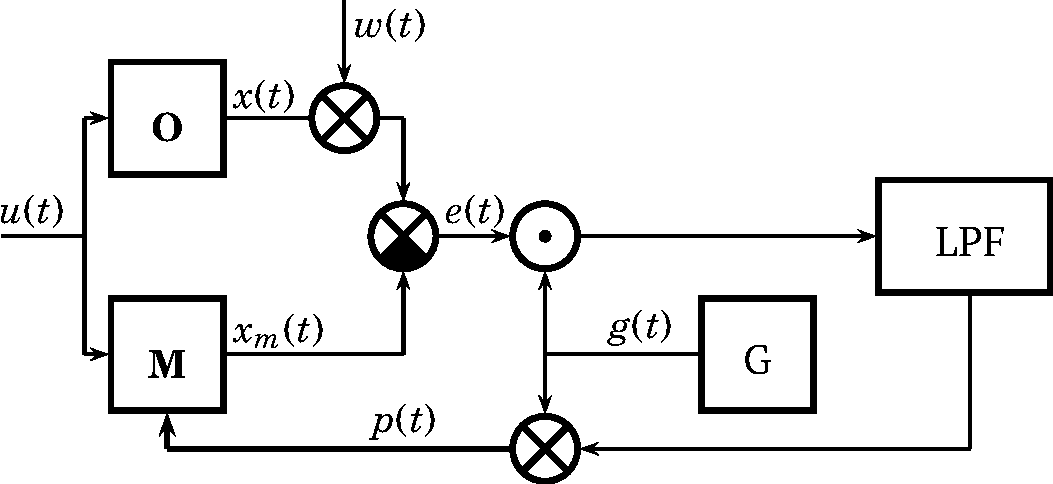
\includegraphics[width=45\TW]{p/oldsch/sd1.png}
      \hfill
      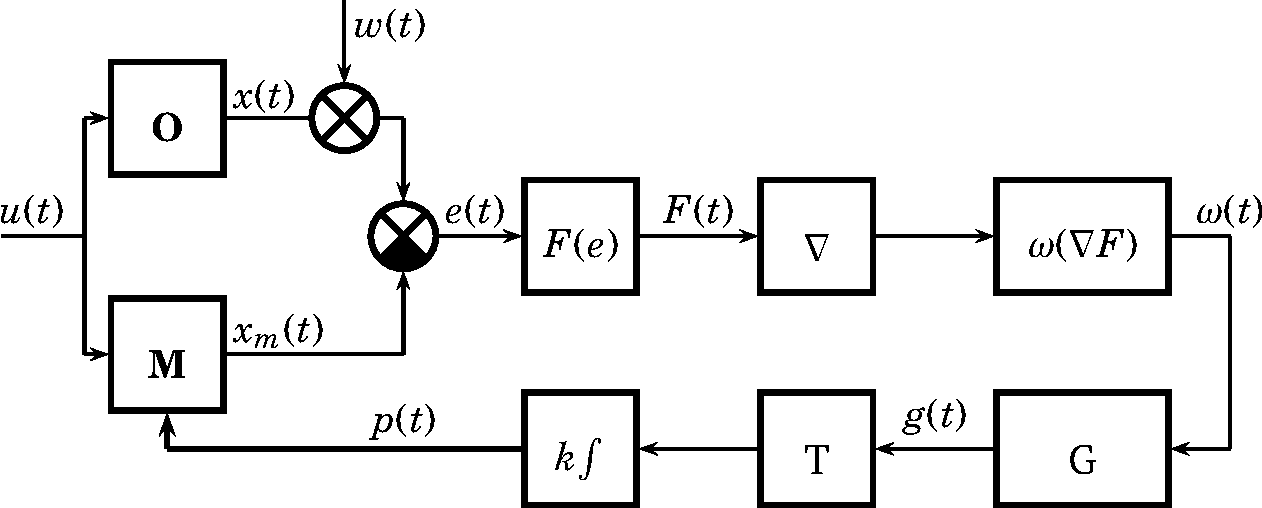
\includegraphics[width=45\TW]{p/oldsch/vsf1.png}
    }
    \centerline{
      {Синхронный детектор}
      \hfill
      {С переменной частотой пробного воздействия}
    }
    \centerline{
      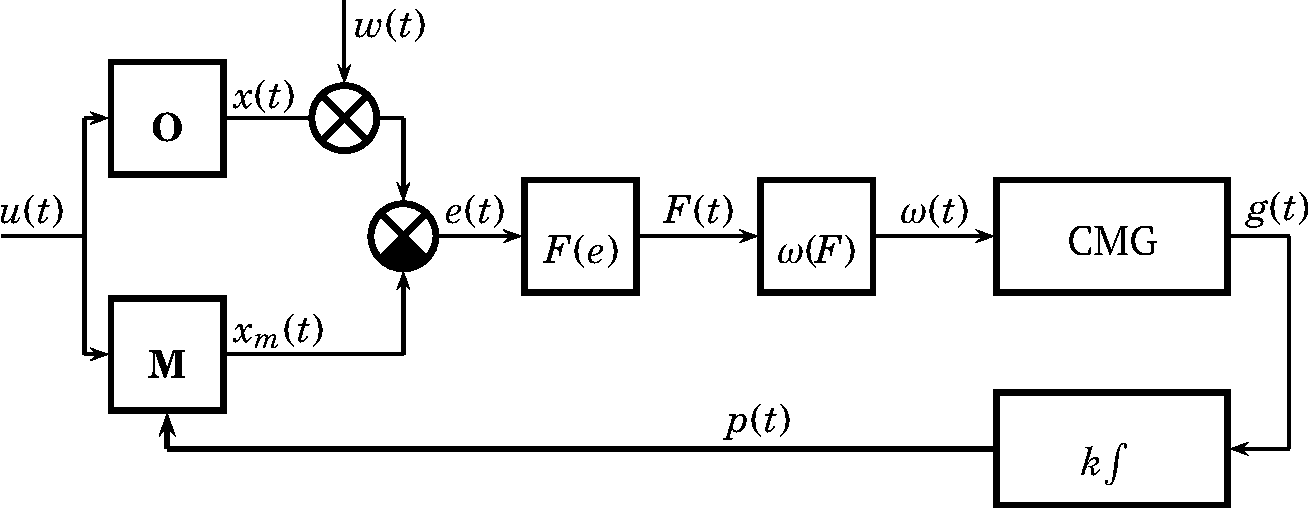
\includegraphics[width=45\TW]{p/oldsch/api1.png}
      \hfill
      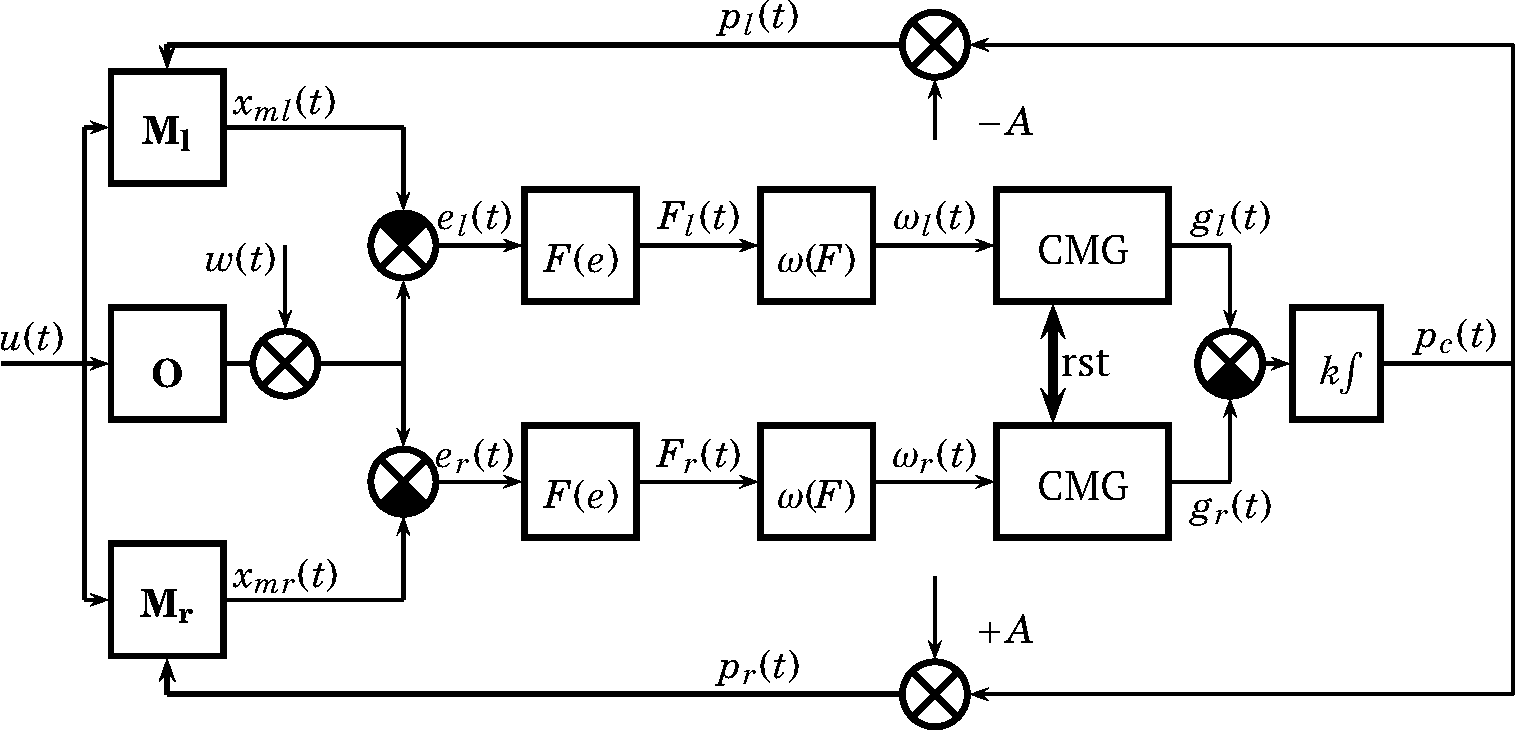
\includegraphics[width=45\TW]{p/oldsch/bimod.png}
    }
    \centerline{
      {Оригинальный адаптивно-поисковый}
      \hfill
      {С  двумя моделями и двумя УГПК}
    }
    \label{atu:f:oldsch}
    \caption{Существующие методы}
  \end{figure}



\end{frame}








% -------------------------- P2 ---------------------------------------------


% ----------------------------- FINAL ------------------------------------------

\begin{frame}
  \frametitle{Научная новизна}
  %\framesubtitle{}

  \noindent
  Впервые:

  \begin{itemize}

    \item
      Предложены \textbf{критерии} идентификации нелинейных динамических систем, которые, в
      отличие от существующих, позволяют оценить их состояние и хаотическую динамику,
      и дают основания для создания эффективных алгоритмов настройки параметров
      моделей систем идентификации.

    \item
      Созданы \textbf{методы} адаптивно-поисковой идентификации на основании
      адаптивно-поисковой парадигмы с использованием \textbf{ансамбля взаимодействующих поисковых агентов},
      и, в отличие от методов, которые
      используют одну модель или пару моделей, значительно повышают скорость поиска и
      способны за минимальное время перестраиваться при резкой смене параметра, а в
      отличие от роевых алгоритмов, новые методы требуют значительно меньшего
      количества моделей и обеспечивают определённые гарантии поиска.

    \item
      Создана новая \textbf{классификация} систем идентификации динамических систем, которая
      как включает в себя как существующие методы, так и позволяет создавать новые методы
      идентификации за счет комбинирования их составных частей.

  \end{itemize}


\end{frame}




% -----------------------------------------------------------------------

\begin{frame}
  \frametitle{Научная новизна (2)}
  %\framesubtitle{}

  \begin{itemize}

    \item
      Установлено, что системы с \textbf{сухим трением} с точки зрения задачи идентификации при
      определенных условиях функционирования обладают свойствами, которые объединяют их с
      системами хаотической динамики, а именно:
      существенная зависимость от начальных условий и вид аттракторов, что
      также требует использования новых методов идентификации.

    \item
      Предложена модель системы хаотической динамики системы
      \textbf{связанных релаксационных генераторов},
      которая отличаешься от существующих отсутствием индуктивных
      компонентов, работоспособностью при малых напряжениях и возможностью управления
      частотным диапазоном в широком диапазоне, что способствует процессу анализа
      хаотической динамики физического объекта, проверки адекватности математической
      модели и свойств системы идентификации на этой системе.

  \end{itemize}

\end{frame}



% -----------------------------------------------------------------------

\begin{frame}
  \frametitle{Научная новизна (3)}
  %\framesubtitle{}

\noindent
Получили дальнейшее развитие:

  \begin{itemize}

    \item
      \textbf{Методы оценки качества идентификации},
      которые в отличие от существующих,
      учитывают использование множества агентов.

    \item
      \textbf{Подходы к адаптации параметров}
      систем адаптивно-поисковой идентификации,
      которые пригодны использовать информацию от ансамбля синергированих моделей, и
      корректировать глобальные параметры поиска.

    \item
      Модель \textbf{генератора Колпитца}, учитывающей большее количество нелинейных эффектов,
      что обеспечивает более адекватные результаты процесса идентификации ее
      параметров новыми методами.

  \end{itemize}


\end{frame}



% -----------------------------------------------------------------------

\begin{frame}
  \frametitle{Практическая ценность}
  %\framesubtitle{}

  \begin{itemize}

    \item
      Разработанные методы идентификации были использованы при проектировании,
      создании, настройке параметров стенда исследования вибрационного и
      акустического воздействия. Анализ результатов данных по этому стенду дал
      возможность указать нужные нелинейные свойства системы, и диапазон параметров,
      в совокупности обеспечивают широкополосный спектр колебаний.

      Науково-практичного дослідження
      ``Оцінка    можливості заміни випробувань КА на стійкість до акустичного навантаження
      випробуваннями широкосмугової вібрації'', згідно договору №~V-105-16-3 від 07.09.2016.

    \item
      Созданное программное среда для моделирования нелинейных динамических систем
      используется при проведении практических работ по дисциплинам
      ``Моделирование систем'', ``Современные системы управления''
      на кафедре информационных технологий
      и систем Национальной металлургической академии Украины.

  \end{itemize}


\end{frame}



% -----------------------------------------------------------------------

\begin{frame}
  \frametitle{Печатные работы и апробация}
  %\framesubtitle{}

По теме диссертации опубликовано
49 печатных работ,
из них
24 входят в международные наукометрические базы,
13 статей опубликовано в материалах конференций.

{\scriptsize
Основные положения диссертационной работы докладывались на
научно-практических конференциях:
``Інформатика та системні науки'' (ІСН-2011) Полтава--2011,
``Интеллектуальные системы принятия решений и проблемы вычислительного интеллекта'' (ISDMCI) Херсон--2011,
``Информационные технологии в управлении сложными системами'' Днепропетровск--2011,
``Автоматизация: проблемы, идеи, решения'' Севастополь--2011,
``Интеллектуальные системы принятия решений и проблемы вычислительного интеллекта'' (ISDMCI) Херсон--2012,
``Автоматизация: проблемы, идеи, решения'' Севастополь--2012,
``Интеллектуальные системы принятия решений и проблемы вычислительного интеллекта'' (ISDMCI) Херсон--2013,
``Автоматизация: проблемы, идеи, решения'' Севастополь--2013,
``Интеллектуальные системы принятия решений и проблемы вычислительного интеллекта'' (ISDMCI) Херсон--2014,
``Интеллектуальные системы принятия решений и проблемы вычислительного интеллекта'' (ISDMCI) Херсон--2015,
``Computer Sciences and Information Technologies'' (CSIT) Lviv--2015 (Scopus),
``Интеллектуальные системы принятия решений и проблемы вычислительного интеллекта'' (ISDMCI) Херсон--2016,
``Data Stream Mining and Processing'' DSMP Lviv--2016 (Scopus,Web of Science).
}

\end{frame}




% -----------------------------------------------------------------------

\begin{frame}
  \frametitle{Выводы}
  %\framesubtitle{}

  \begin{itemize}

    \item[---]
      Созданы новые критерии идентификации,
      пригодные для анализа состояния и динамики хаотических систем, что создаёт
      физическое  обоснование для создания работоспособных систем идентификации.

    \item
      Создан новый класс систем идентификации в рамках адаптивно-поисковом парадигмы,
      которые за счет использования коллективной динамики ансамбля поисковых
      агентов обеспечивают лучшее качество идентификации.

    \item
      Создано программное обеспечение, пригодное для моделирования как систем
      хаотической динамики, так и систем мультиагентной идентификации.

    \item
      Проведено компьютерное моделирование процессов идентификации систем хаотической
      динамики, подтверждена их работоспособность.

  \end{itemize}

  \begin{example}
    exa
  \end{example}


  \begin{alertblock}{alert}
    alert1
  \end{alertblock}


  \begin{block}{Block}
    Block1
  \end{block}



\end{frame}



% -----------------------------------------------------------------------
%
% \begin{frame}
%   \frametitle{Выводы 2}
%   %\framesubtitle{}
%
%
% \end{frame}



\end{document}

